\documentclass[11pt,a4paper]{article}
\usepackage[utf8]{inputenc}
\usepackage[T1]{fontenc}
\usepackage{amsmath,amssymb,geometry,booktabs,graphicx,xcolor,array}
\usepackage{lmodern}
\usepackage[skip=4pt]{caption}
\geometry{margin=2cm}
\setlength{\parindent}{0pt}
\setlength{\parskip}{5pt}
\definecolor{joint}{HTML}{f07167}
\definecolor{jac}{HTML}{0081a7}
\newcommand{\summarybox}[1]{\fcolorbox{gray}{gray!6}{\parbox{0.96\linewidth}{#1}}}

\title{Straight-path cost for the FL controller:\\ joint-line cost vs.\ Jacobian cost}
\author{WP1 \quad--\quad \texttt{Controllers/FL.py}, \texttt{Final\_Code/path\_constraint\_jacobian.py}}
\date{}

\begin{document}
\maketitle
\vspace{-0.8cm}

\summarybox{\textbf{In one line.} Both methods add a quadratic path term $x_t^\top Q^{\rm path}_t x_t$ to the
same FL LQG problem. \textcolor{joint}{\textbf{Yours}} penalises the distance to a \emph{straight
line in joint space}, mostly in the last 50\,ms. \textcolor{jac}{\textbf{The Jacobian cost}}
penalises the hand's \emph{actual distance to the straight hand line}, linearised with $J(\theta)$,
at every step. Same simulation, same weights, only $Q^{\rm path}_t$ changes.}

%-------------------------------------------------------------------------------
\section{Common setting: the FL controller}

\textbf{State} ($8$): angles, velocities, target angles, start angles
\[
x=\big[\theta_s,\ \theta_e,\ \omega_s,\ \omega_e,\ \theta_s^{\rm tg},\ \theta_e^{\rm tg},\
\theta_s^{0},\ \theta_e^{0}\big]^\top .
\]
\textbf{Feedback linearisation} turns the arm into a double integrator, $\ddot\theta = v$, so with
$\Delta t=10$\,ms, $N=60$ steps:
\[
x_{t+1}=A\,x_t+B\,v_t,\qquad
A=\mathbb I_8 + \Delta t\,(e_1e_3^\top+e_2e_4^\top),\qquad B=\Delta t\,(e_3e_1^\top+e_4e_2^\top).
\]
\textbf{Cost} (weights of \texttt{common.py}: $w_p=2\cdot10^4$, $w_v=10$, $r=6\cdot10^{-5}$):
\[
\mathcal J=\underbrace{w_p\|\theta_N-\theta^{\rm tg}\|^2+w_v\|\omega_N\|^2}_{x_N^\top Q_f\,x_N}
\;+\;\sum_{t=0}^{N-1}\Big(\underbrace{x_t^\top Q^{\rm path}_t\,x_t}_{\text{path term}}
+\;r\,\|v_t\|^2\Big).
\]
\textbf{Riccati} ($S_N=Q_f$, backwards in $t$) and \textbf{command}:
\[
L_t=\big(rI+B^\top S_{t+1}B\big)^{-1}B^\top S_{t+1}A,\qquad
S_t=Q^{\rm path}_t+A^\top S_{t+1}(A-BL_t),\qquad v_t=-L_t\,\hat x_t ,
\]
\[
u_t=\big(\mathcal A\,{\rm diag}(f_l f_v)\big)^{+}\big(M(\theta)\,v_t+C(\theta,\omega)+B_{\rm visc}\,\omega\big),
\]
with $\hat x_t$ the Kalman estimate (60\,ms delay), $\mathcal A$ the moment arms, $f_l,f_v$ the
force--length and force--velocity gains. \emph{Everything here is shared}; the two methods only
differ in $Q^{\rm path}_t$.

%-------------------------------------------------------------------------------
\section{\textcolor{joint}{Your method}: joint-line cost (\texttt{compute\_path})}

\textbf{1. A line in joint space.} Take the hand point $75\%$ of the way,
$p^{\rm ref}=p_0+0.75\,(p_f-p_0)$, its posture $\theta^{\rm ref}={\rm IK}(p^{\rm ref})$, and the slope
\[
k=\frac{\theta_e^{\rm ref}-\theta_e^{0}}{\theta_s^{\rm ref}-\theta_s^{0}} .
\]
\textbf{2. Distance to that line} (linear in $x$, uses the start angles stored in the state):
\[
d_J(x)=k\,(\theta_s-\theta_s^{0})-(\theta_e-\theta_e^{0})=h^\top x,\qquad
h=[\,k,\ -1,\ 0,\ 0,\ 0,\ 0,\ -k,\ 1\,]^\top .
\]
\textbf{3. Path term}, end-loaded with $\tau=0.02$\,s:
\[
\boxed{\;Q^{\rm path}_t=w_c\,e^{-(N-1-t)\Delta t/\tau}\;h\,h^\top\qquad
\Rightarrow\quad x_t^\top Q^{\rm path}_tx_t=w_c\,e^{-(N-1-t)\Delta t/\tau}\,d_J(x_t)^2\;}
\]
Each step back from the end divides the weight by $e^{0.5}\approx1.65$: the last 5 steps
(50\,ms) carry $92\%$ of it.

\begin{figure}[h]
\centering
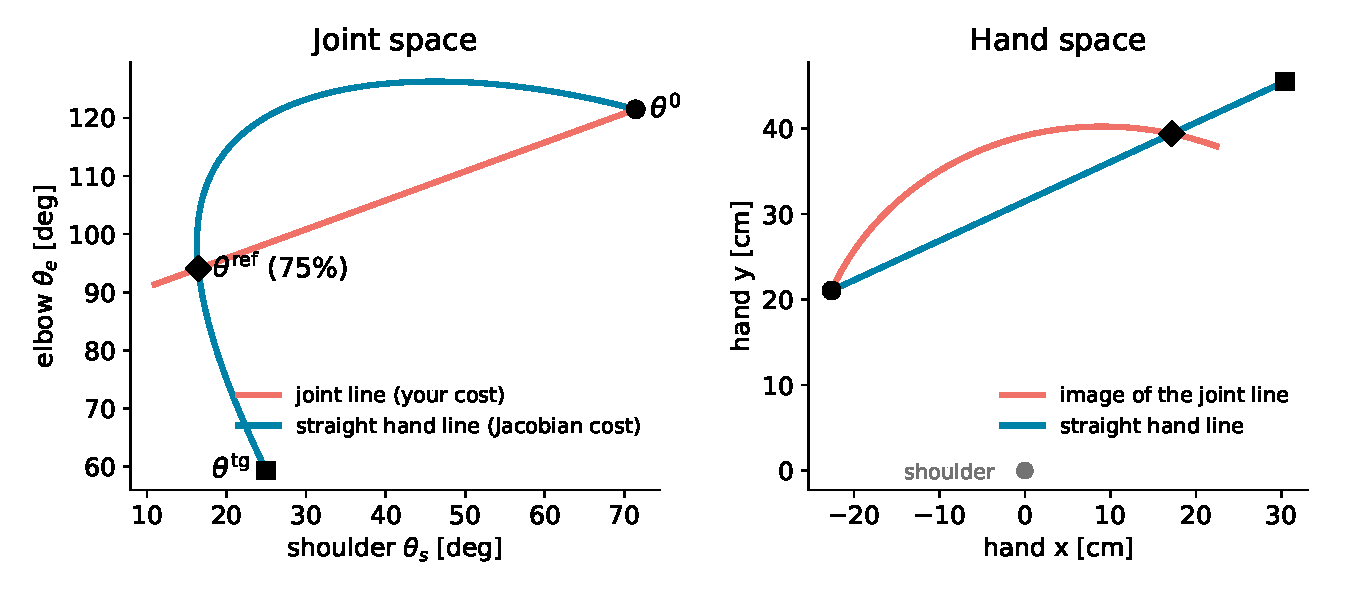
\includegraphics[width=\linewidth]{fig_geometry.pdf}
\caption{Movement 1. \textcolor{joint}{Your joint line} (through $\theta^0$ and $\theta^{\rm ref}$)
is straight in joint space but curved for the hand, and it does not pass through the target
$\theta^{\rm tg}$. \textcolor{jac}{The straight hand line} is curved in joint space.
$k=0.50$.}
\end{figure}

\textbf{Consequences.}
\begin{itemize}\setlength\itemsep{1pt}
\item Exact quadratic, no approximation, very cheap.
\item But a \emph{proxy}: a straight joint line is not a straight hand path (Fig.~1, right).
\item The line misses the target, and the cost acts at the end: it pulls against reaching
$\theta^{\rm tg}$ at rest $\Rightarrow$ late correction, higher terminal and peak velocities.
\item Straightening stops around $w_c\approx80$--$100$ (1.8--2.7\,cm); above, the path curves again.
\end{itemize}

%-------------------------------------------------------------------------------
\section{\textcolor{jac}{Jacobian method}: quadratised hand deviation}

\textbf{1. The quantity we actually want small:} the lateral distance of the hand to the line.
\[
p(\theta)=\begin{bmatrix} l_1\cos\theta_s+l_2\cos(\theta_s+\theta_e)\\ l_1\sin\theta_s+l_2\sin(\theta_s+\theta_e)\end{bmatrix},
\qquad
a=\frac{p_f-p_0}{\|p_f-p_0\|},\quad n=\begin{bmatrix}-a_y\\ a_x\end{bmatrix},
\qquad
\boxed{\;e(\theta)=n^\top\big(p(\theta)-p_0\big)\;}
\]
$e$ is \emph{not} quadratic in $\theta$ $\Rightarrow$ linearise it.

\textbf{2. Linearise at a posture on the line.} Pick $\theta^*_t$ with $p(\theta^*_t)$ on the line,
so $e(\theta^*_t)=0$:
\[
e(\theta)\;\approx\;n^\top J(\theta^*_t)\,(\theta-\theta^*_t)=g_t^\top\theta-c_t,
\qquad g_t=J(\theta^*_t)^\top n,\quad c_t=g_t^\top\theta^*_t,
\]
\[
J(\theta)=\begin{bmatrix}-l_1\sin\theta_s-l_2\sin(\theta_s+\theta_e) & -l_2\sin(\theta_s+\theta_e)\\
l_1\cos\theta_s+l_2\cos(\theta_s+\theta_e) & l_2\cos(\theta_s+\theta_e)\end{bmatrix}.
\]
The error is second order in $\theta-\theta^*_t$, and the cost itself keeps $\theta$ close to the line.

\textbf{3. Make it quadratic: add a constant state.} $g_t^\top\theta-c_t$ is affine, so use
$z=[x;\,1]$ ($9$ states):
\[
\boxed{\;Q^{\rm path}_t=w_J\,h_th_t^\top,\qquad h_t=[\,g_t^\top,\ 0_{1\times6},\ -c_t\,]^\top
\qquad\Rightarrow\quad z_t^\top Q^{\rm path}_tz_t=w_J\,(g_t^\top\theta_t-c_t)^2\;}
\]
\[
A_z=\begin{bmatrix}A&0\\0&1\end{bmatrix},\quad B_z=\begin{bmatrix}B\\0\end{bmatrix},\quad
\text{same Riccati}\ \Rightarrow\ v_t=-L_t\begin{bmatrix}\hat x_t\\1\end{bmatrix}
=-L^x_t\hat x_t-\ell_t\quad\text{(affine feedback)}.
\]
\emph{Uniform in time}: every step is penalised equally.

\textbf{4. Where to linearise ($\theta^*_t$).} Start from a minimum-jerk progress along the line,
\[
s(\tau)=10\tau^3-15\tau^4+6\tau^5,\qquad \theta^*_t={\rm IK}\big(p_0+s(t/N)\,(p_f-p_0)\big),
\]
then optionally re-linearise: run the noiseless controller, project its hand path onto the line,
recompute $\theta^*_t$ (3 times). Here it barely matters: the linearised deviation is within $5\%$
of the real one even $12$\,cm off the line, and exact to $<0.05$\,cm once straight.

%-------------------------------------------------------------------------------
\section{Side by side}

\begin{center}
\renewcommand{\arraystretch}{1.25}
\begin{tabular}{>{\raggedright}p{3.0cm}>{\raggedright}p{5.4cm}>{\raggedright\arraybackslash}p{5.6cm}}
\toprule
 & \textcolor{joint}{\textbf{Joint-line (yours)}} & \textcolor{jac}{\textbf{Jacobian}}\\
\midrule
Penalised quantity & $d_J=k(\theta_s-\theta_s^0)-(\theta_e-\theta_e^0)$ & $e\approx g_t^\top\theta-c_t$, hand distance to the line\\
Space & joint (proxy) & hand (the real target)\\
Exact? & exact quadratic of a proxy & first-order approximation of the real quantity\\
When & last $\sim$50\,ms ($e^{-\text{time to go}/\tau}$) & every step, uniform\\
Matrix & fixed $h\,h^\top$ & time-varying $h_th_t^\top$\\
State & 8 & 9 (constant $1$, affine feedback)\\
Needs & IK of one point & IK along the line, a reference timing\\
Weight range used & $w_c\in\{0,\dots,80\}$ (rad$^2$) & $w_J\in\{0,\dots,0.01\}$ (cm$^2$)\\
\bottomrule
\end{tabular}
\end{center}

%-------------------------------------------------------------------------------
\section{Results (two 58\,cm movements, 600\,ms)}

\begin{figure}[h]
\centering
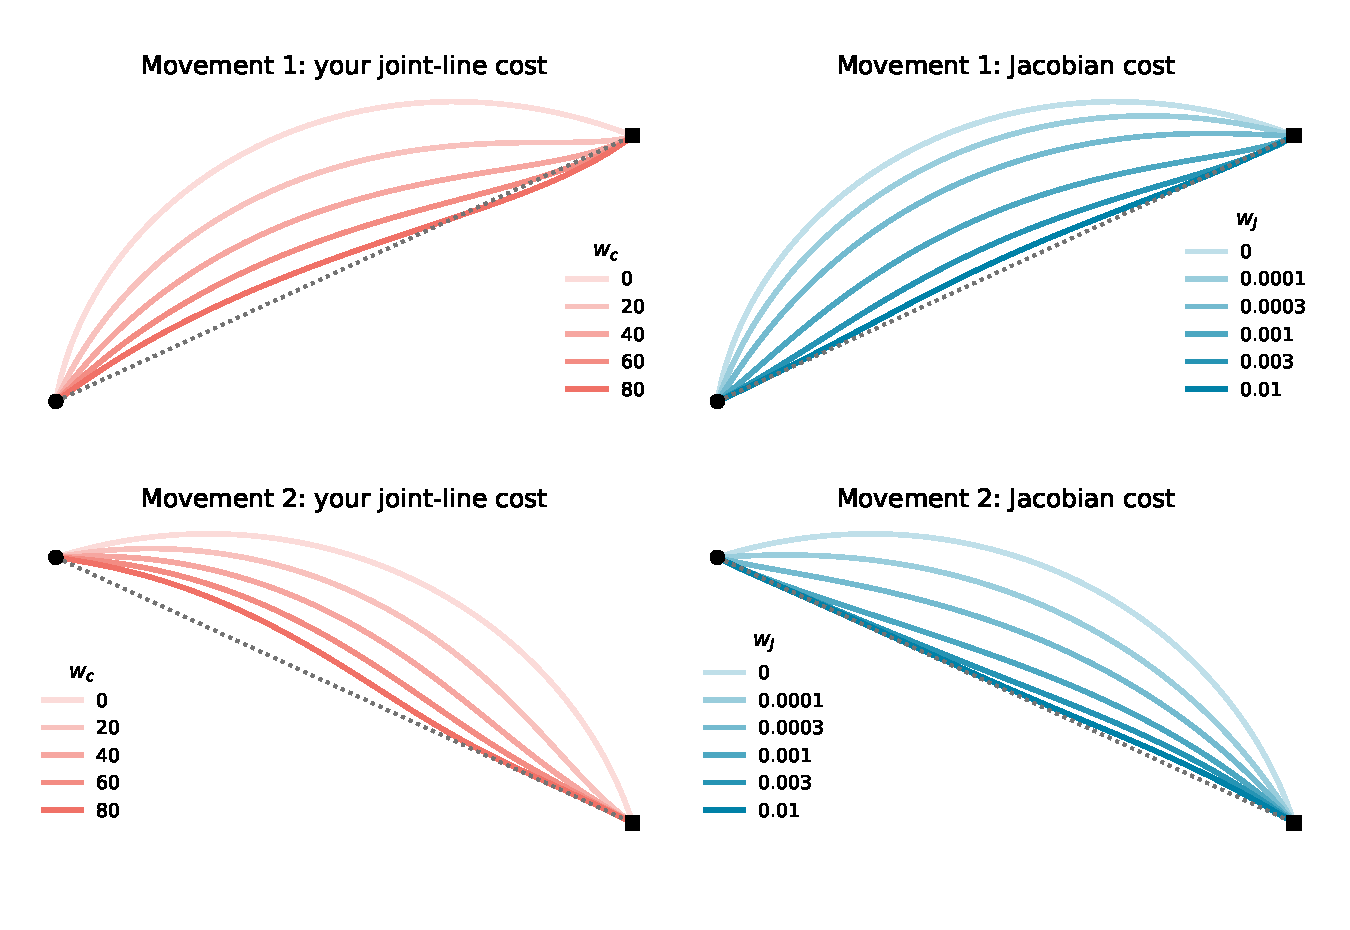
\includegraphics[width=0.85\linewidth]{fig_paths.pdf}
\caption{Noiseless hand paths over each weight sweep (light $\to$ dark = more weight).
Jacobian gains with 3 re-linearisations; without them the paths differ by less than 0.6\,cm.}
\end{figure}

\noindent\begin{minipage}{\linewidth}
\textbf{At matched straightness} (200 noisy trials each; your straightest setting $w_c=80$):

\begin{center}
\small
\renewcommand{\arraystretch}{1.15}
\begin{tabular}{lccccc}
\toprule
 & lateral dev. & terminal vel. & peak vel. & effort $\sum u^2$ & movement cost\\
\midrule
Mvt 1, \textcolor{joint}{$w_c=80$} & 1.8 cm & 12.0 °/s & 346 °/s & 32.2 & 5.06\\
Mvt 1, \textcolor{jac}{$w_J=0.003$} & 2.6 cm & \textbf{4.2} °/s & \textbf{227} °/s & 32.7 & \textbf{3.79}\\
Mvt 1, \textcolor{jac}{$w_J=0.01$} & \textbf{1.0} cm & \textbf{3.8} °/s & 241 °/s & 35.6 & 4.05\\
\midrule
Mvt 2, \textcolor{joint}{$w_c=80$} & 2.7 cm & 6.7 °/s & 234 °/s & 59.0 & 6.77\\
Mvt 2, \textcolor{jac}{$w_J=0.003$} & \textbf{1.6} cm & \textbf{4.0} °/s & 263 °/s & \textbf{34.7} & \textbf{3.96}\\
\midrule
No path cost (mvt 1 / 2) & 13.6 / 12.0 cm & $\sim$3.9 °/s & 157 / 254 °/s & 26.7 / 55.2 & 3.19 / 6.02\\
\bottomrule
\end{tabular}
\end{center}
\end{minipage}

\begin{itemize}\setlength\itemsep{1pt}
\item \textbf{Straighter:} down to 1.0 / 0.75\,cm noisy, $<0.1$\,cm noiseless (yours stops at 1.8 / 2.7\,cm).
\item \textbf{Stops at the target:} terminal velocity at the noise floor ($\sim$4\,°/s, as with no
path cost). Endpoint error is the same for all ($\sim$0.15--0.20\,cm).
\item \textbf{Smoother} on mvt 1 (peak 227 vs 346\,°/s), \textbf{41\% less effort} on mvt 2.
\end{itemize}

\begin{figure}[h]
\centering
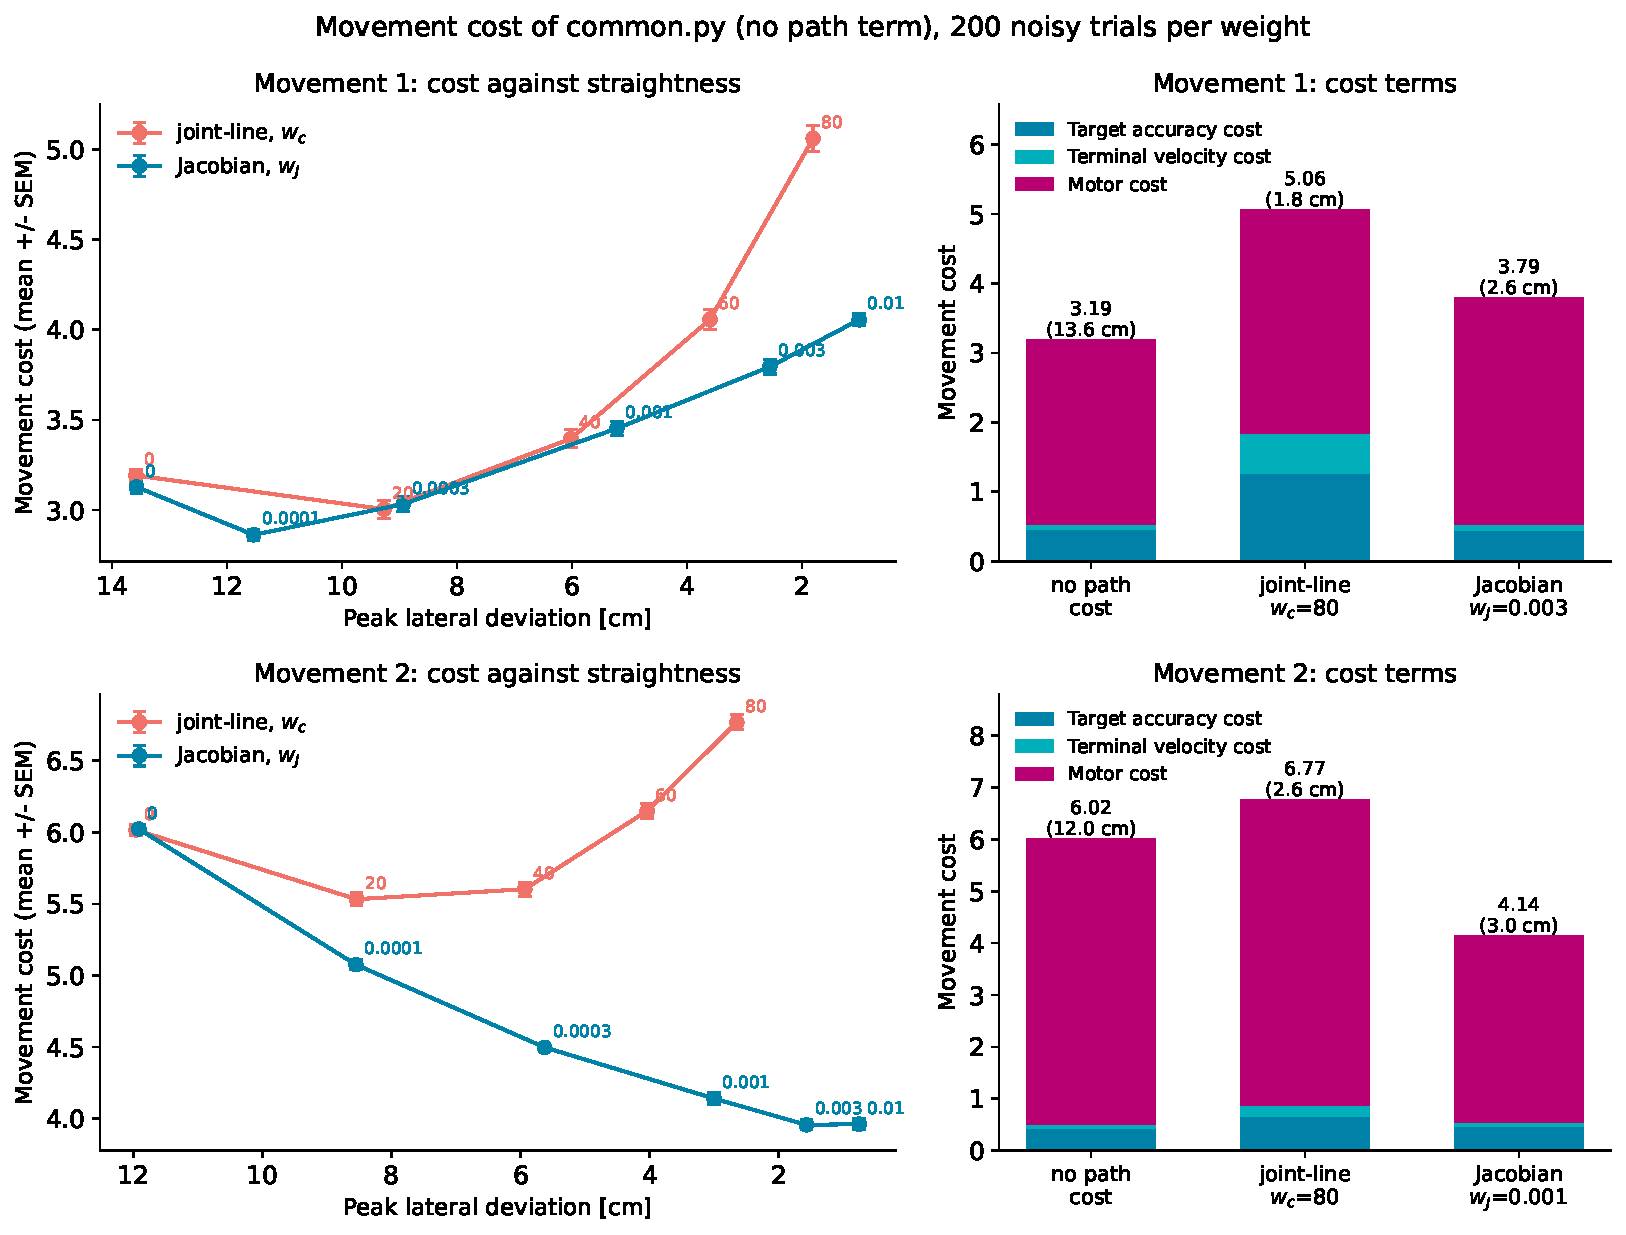
\includegraphics[width=0.95\linewidth]{fig_cost.pdf}
\caption{Movement cost of \texttt{common.py}: $w_p\|\theta_N-\theta^{\rm tg}\|^2+w_v\|\omega_N\|^2
+0.1\sum_t\|u_t\|^2$ (muscle commands), without the path term, which differs between methods.}
\end{figure}

\textbf{Movement cost.}
\begin{itemize}\setlength\itemsep{1pt}
\item \textcolor{joint}{Yours} makes straight paths expensive: $+59\%$ (mvt 1) and $+12\%$ (mvt 2)
over no path cost. The end-loaded term fights the arrival: accuracy cost $\times2.8$, terminal
velocity cost $\times7.7$ on mvt 1.
\item \textcolor{jac}{Jacobian} keeps accuracy and terminal velocity at their no-path level; only the
motor term moves: $+19\%$ in total for mvt 1 (at 2.6\,cm), $\mathbf{-31\%}$ to $\mathbf{-34\%}$
for mvt 2 (at 3.0 to 1.6\,cm), where the straight path is \emph{cheaper} than the FL default path.
\end{itemize}

\noindent\begin{minipage}{\linewidth}
\textbf{Simulation time} (one core, per movement; per-trial runs are identical):

\begin{center}
\renewcommand{\arraystretch}{1.15}
\begin{tabular}{lcc}
\toprule
 & \textcolor{joint}{Joint-line} & \textcolor{jac}{Jacobian}\\
\midrule
Gains, once per weight & 1.8 ms & 3.6 ms (no re-linearisation)\\
 & & 83 ms (3 re-linearisations)\\
One noisy trial (60 steps, Kalman with delay) & 17.5 ms & 17.5 ms\\
200 trials, one weight & 3.50 s & 3.50 s / 3.58 s ($+2\%$)\\
\bottomrule
\end{tabular}
\end{center}
\end{minipage}

The per-step Kalman filter dominates; the Riccati recursion is under $10\%$.
For reference, \texttt{run\_fl} (used by \texttt{path\_constraint.py}) recomputes the gains
on every trial: 18.8\,ms per trial.

%-------------------------------------------------------------------------------
\section{Limitations of the Jacobian method}
\begin{itemize}\setlength\itemsep{1pt}
\item \textbf{First order only.} It minimises the \emph{linearised} deviation. Small here
($\le5\%$), but it would grow for highly curved maps or very weak weights.
\item \textbf{Needs a reference timing} $\theta^*_t$. Gains are computed offline: a large
perturbation that delays or advances the hand (e.g.\ a force field) moves the linearisation point.
Not tested.
\item \textbf{The whole line must be reachable} and away from singularities ($\det J\neq0$).
Here the elbow stays within $59^\circ$--$126^\circ$; a line near the shoulder or at full extension fails.
\item \textbf{One extra state} (the constant $1$): \texttt{simulate\_FL} is written for 8 states,
so the script uses its own copy of the loop (it reproduces \texttt{simulate\_FL} exactly).
\item \textbf{Weights not comparable} with $w_c$ (cm$^2$ vs rad$^2$): compare at equal straightness.
\end{itemize}

\end{document}
